\documentclass[11pt]{report}

% Paquetes y configuraciones adicionales
\usepackage{graphicx}
\usepackage[export]{adjustbox}
\usepackage{caption}
\usepackage{float}
\usepackage{titlesec}
\usepackage{geometry}
\usepackage[hidelinks]{hyperref}
\usepackage{parskip}
\usepackage{fontspec}

% Configuración de la fuente usada
\setmainfont{Geist}


% Configura los márgenes
\geometry{
    left=2cm,   % Ajusta este valor al margen izquierdo deseado
    right=2cm,  % Ajusta este valor al margen derecho deseado
    top=2cm,
    bottom=2cm,
}

% Redefinir el formato del capítulo
\titleformat{\chapter}[block]
  {\normalfont\huge\bfseries}{\chaptertitlename\ \thechapter}{1em}{\Huge}

% Ajustar el espaciado antes y después del título del capítulo
\titlespacing*{\chapter}{0pt}{0pt}{20pt}

% Configuración de los títulos de las secciones
\titlespacing{\section}{0pt}{\parskip}{\parskip}
\titlespacing{\subsection}{0pt}{\parskip}{\parskip}
\titlespacing{\subsubsection}{0pt}{\parskip}{\parskip}


\begin{document}
	
	% Portada del informe
	
	\title{Linked Data}
	\author{Samuel Martín Morales  \texttt{alu0101359526@ull.edu.es} \and Jorge Domínguez González  \texttt{alu0101330600@ull.edu.es} \and Juan Diego Rendon Cachafeiro \texttt{alu0101327747@ull.edu.es}}
	\date{\today}
	
	\maketitle
	
	% Índice
	\tableofcontents
	
	% Secciones del informe
	\chapter{Introducción}

  En la última década, la web ha experimentado una transformación fundamental desde una simple red de información hacia lo que hoy se conoce como \textbf{Linked Data} o \textbf{datos enlazados}. Este cambio, impulsado por la evolución de la web semántica, ha llevado a la adopción de un paradigma que va más allá de la  presentación de información en forma de texto. Linked Data propone una visión donde los datos adquieren una estructura que facilita la creación de conexiones y enlaces entre diversos conjuntos de datos, provenientes incluso de fuentes y proveedores distintos.

De manera general, Linked Data representa un conjunto de prácticas sólidas para la publicación y conexión de datos estructurados en la web. Haciendo uso de tecnologías del W3C, como \textbf{URIs}, el \textbf{protocolo HTTP} y el modelo de datos \textbf{RDF} o \texttt{\textbf{Resource Description Framework}}, se establece una base que permite la identificación única de entidades, la recuperación de recursos y la descripción detallada de los mismos.

En el presente informe se tiene como objetivo explorar los fundamentos de Linked Data, desde sus principios esenciales hasta su aplicación práctica. En esencia este se centrará en cómo las URIs, el protocolo HTTP y el modelo RDF forman parte de la revolución semántica, permitiendo la interconexión de datos. Además, se examinará el impacto del Linked Open Data (LOD) y cómo este enfoque híbrido entre \texttt{datos enlazados} y \texttt{datos abiertos} está transformando la forma en la que se accede, se utiliza y se comparte la información en un mundo cada vez más interconectado.
	 
	\chapter{Componentes del Linked Data}

	Para comenzar con el estudio de Linked Data, es necesario entender los componentes que lo conforman. En este sentido, se puede decir que Linked Data se basa en tres pilares fundamentales: URIs, HTTP y RDF. A continuación, se describirá cada uno de estos componentes y se explicará su importancia en el contexto de Linked Data.

- URI (Identificadores de recursos uniformes): Una URI es una cadena de caracteres que identifica de manera única un recurso en la web. En este perspectiva, se puede decir que una URI es un identificador de recursos uniforme, ya que, permite la identificación de los distintos recursos en la web de una manera uniforme y consistente. Además, las URIs son utilizadas por los agentes de software para acceder a los recursos de esta. La uniformidad en el contexto de las URIs hace referencia a los siguiente aspectos:

\indent \indent \indent -  \textbf{Unicidad}: Cada recurso debe tener una URI única. La unicidad garantiza que no haya conflictos ni duplicados en la identificación de los recursos. Cada URI debería de ser única en el ámbito global de la web.

\indent \indent \indent -  \textbf{Consistencia}: Las URIS deben de seguir un formato consistente y estandarizado. Esto permite la facilidad de comprensión y manejo por parte tanto de las máquinas como de las personas. Además, permite el establecimiento de patrones y la simplificación de su uso.

\indent \indent \indent -  \textbf{Persistencia}: Las URIs deben de ser persistentes. Esto quiere decir que una URI debe de ser válida y accesible en todo momento. De esta manera, se garantiza que los recursos puedan ser accedidos en el momento que se considere.

\indent \indent \indent -  \textbf{Desreferenciable}: Las URIs deben de ser desreferenciables. Es decir, el acceder a una URI mediante el protocolo \texttt{HTTP} se debe de obtener información sobre el recurso al que hace referencia la URI. Esto permite que las URIs no solo se traten de identificadores únicos, sino 	que también sean enlaces a información relevante.

- HTTP (Protocolo de Transferencia de Hipertexto): Se hace uso del protocolo HTTP para que las URIs sean desreferenciables. Esto quiere decir que, al acceder a una URI mediante el protocolo HTTP se debe de obtener información sobre el recurso al que hace referencia la URI. Además, el protocolo HTTP permite la recuperación de recursos a través de la web. En este sentido, se puede decir que el protocolo HTTP es el protocolo de la web, ya que, es el protocolo que permite la recuperación de recursos a través de esta. En cuanto a las características del protocolo, se pueden encontrar las siguientes a continuación:

\indent \indent \indent - \textbf{Cliente-Servidor}: El protocolo HTTP se basa en un modelo cliente-servidor. Esto quiere decir que, el cliente realiza una petición al servidor y este le responde con la información solicitada. En este sentido, el cliente es el agente de software que realiza la petición y el servidor es el agente de software que responde a la petición.

\indent \indent \indent - \textbf{Sin estado}: El protocolo HTTP es un protocolo sin estado. Es decir, cada petición que se realiza al servidor es independiente de las demás. Por tanto, el servidor no guarda información sobre las peticiones anteriores. Esto permite que el protocolo sea simple y fácil de implementar.

\indent \indent \indent - \textbf{Protocolo de aplicación}: Se trata de un protocolo de nivel de aplicación utilizado para la transferencia de información en la WWW (\texttt{World Wide Web}). De manera general, opera en la capa de aplicación del modelo OSI (\texttt{Open Systems Interconnection}) \cite{1}. 

\indent \indent \indent - \textbf{Mensajes}: Las comunicaciones se realizan mediante mensajes. Un solicitud de un cliente y una respuesta del servidor consisten en un encabezado y de manera opcional en un cuerpo. El encabezado contiene la información sobre dicha solicitud o respuesta y el cuerpo contiene la infomación que se quiere transmitir.

\indent \indent \indent - \textbf{URis}: Las distintas solicitudes y respuestas en HTTP hacen uso de identificadores de recursos uniformes para identificar los distintos recursos en la web. Esto lo que permite, es especificar la ubicación y el nombre del recurso.

\indent \indent \indent - \textbf{Basado en texto}: Las distintas solicitudes y respuestas se codifican en texto.  Esto lo que permite es que se facilita la comprensión y el procesamiento de las solicitudes y respuestas tanto por parte de los humanos como de las propias máquinas.

\indent \indent \indent - \textbf{Métodos}: El protocolo define una serie de métodos que se utilizan para poder indicar la acción que el cliente quiere realizar. Algunos de los métodos más comunes son GET, POST, PUT, DELETE, etc.

- RDF (Marco de Descripción de Recursos): RDF es un modelo estándar para describir recursos y sus relaciones haciendo uso de tripletes (sujeto, predicado, objeto).

\indent \indent \indent - \textbf{Reutilización}: RDF hace uso de URIs para identificar los recursos, permitiendo la facilidad en la reutilización de la información RDF en diferentes aplicaciones.

\indent \indent \indent - \textbf{Interoperabilidad}: Este está estandarizado por el W3C \cite{5}, lo que permite que diferentes aplicaciones RDF puedan trabajar juntas más fácilmente.

\indent \indent \indent - \textbf{Extensibilidad}: RDF permite la extensión de vocabularios RDF existentes, lo que permite la creación de vocabularios RDF más específicos.

\indent \indent \indent - \textbf{Escalabilidad}: Se puede hacer más grande según sea necesario (escalable),  permitiendo que se pueda usar para representar grandes cantidades de información o datos.

- Enlaces entre recursos: Las URIs deben de incluir enlances (enlaces de hipertexto) a otras URIs, de esta manera se pueden establecer relaciones entre los recursos y la navegación entre estos. Esto lo que permite es la fomentación de la creación de una red interconectada de datos en la web.

Estos componentes permiten que los datos estén interconectados, facilitando por un lado la navegación y el descubrimiento de información relacionada. Por tanto, cuando se siguen estos principios, se puede decir que los datos están enlazados (\textbf{Linked Data}), siendo estos datos fundamentales para la construcción de la web semántica, dónde, la información tiene un significado definido y las máquinas pueden entender y procesar los datos de manera efectiva.

Teniendo en cuenta todo esto anterior, se puede observar a continuación una esquema de todo lo comentado anteriormente, de tal manera que los conceptos básicos puedan ser comprendidos de manera más sencilla \ref{fig:Componentes-Linked-Data}.

\begin{figure}[H]
	\centering
	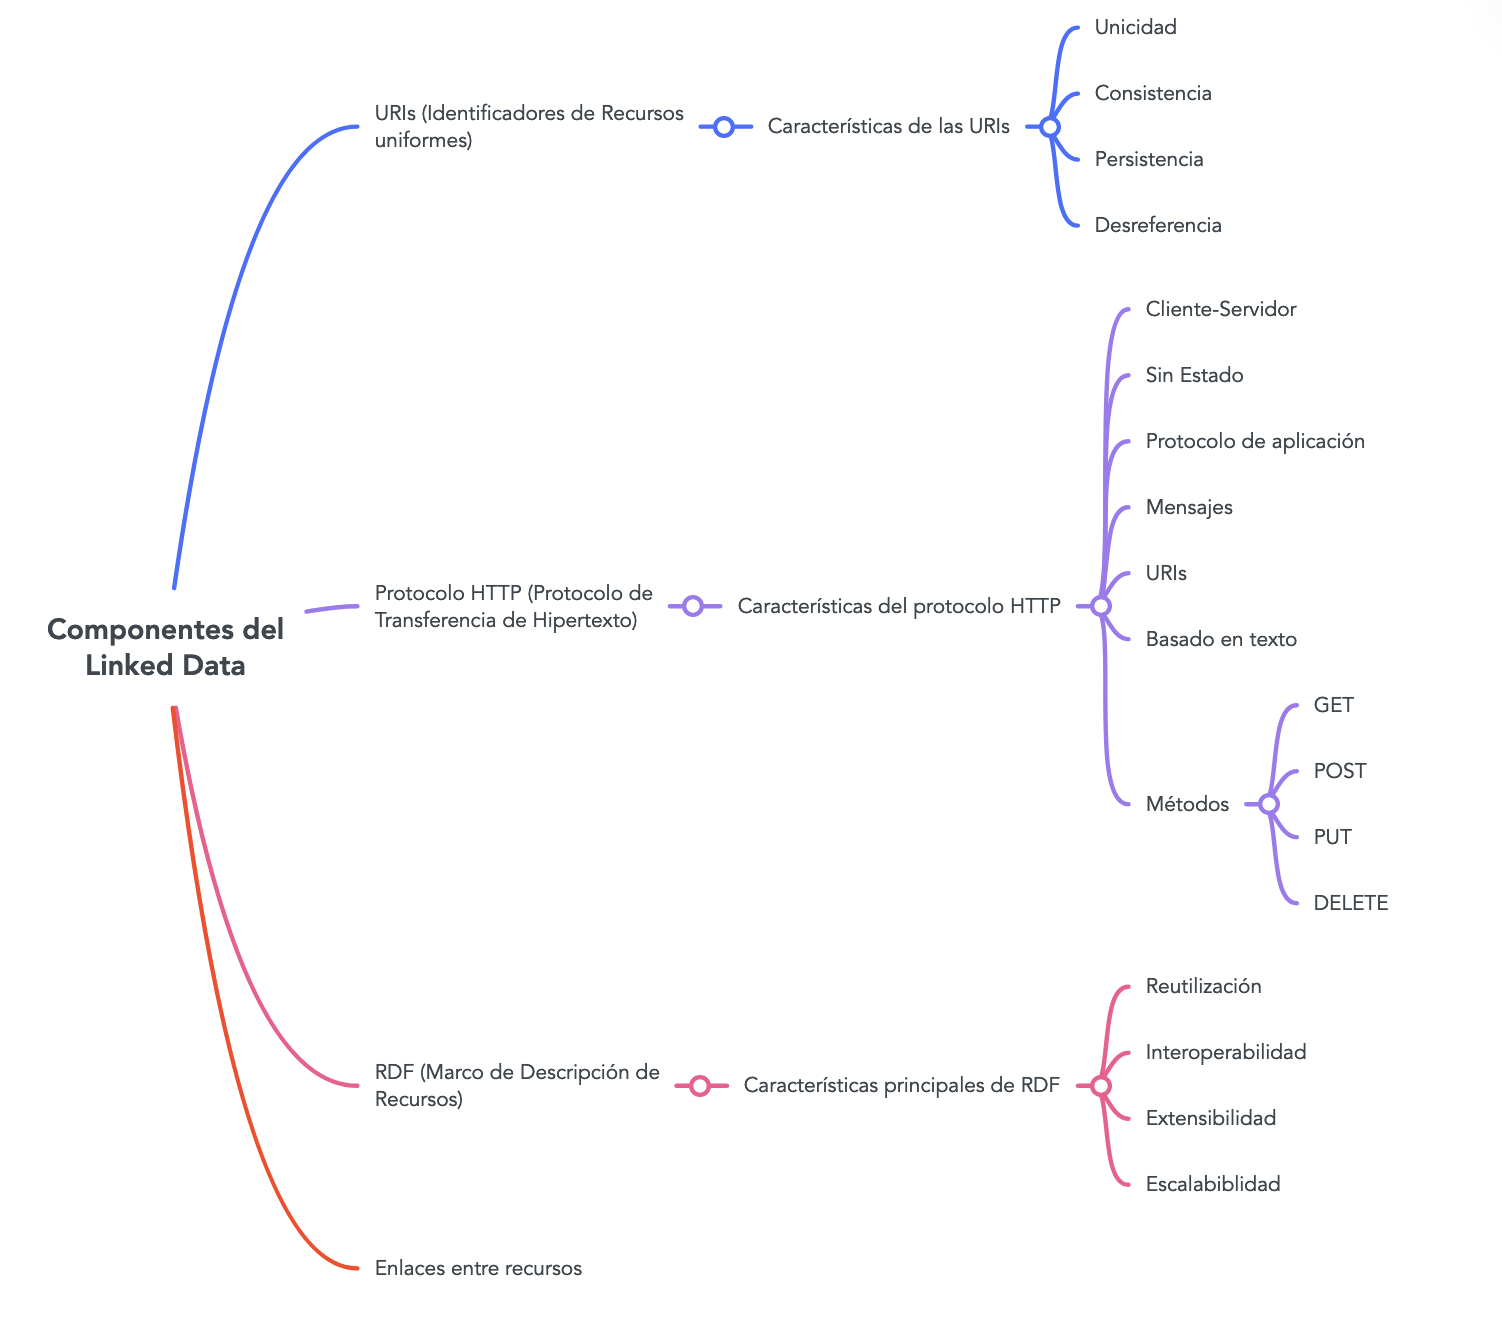
\includegraphics[scale=0.6]{../img/Componentes-Linked-Data.png}
	\caption{Esquema de los principales componentes de Linked Data..}
	\label{fig:Componentes-Linked-Data}
\end{figure}

	\chapter{RDF de manera básica}
  Como se ha comentado de manera previa, \texttt{RDF} es un \textbf{modelo} que permite representar propiedades y valores de propiedades. Este, se basa en principios que se encuentran establecidos haciendo uso de varios tipos de representación de datos. Por otro lado, se puede hablar de las \textbf{propiedades RDF}, estas, se asemejan a los atributos y de manera general se corresponden con los pares de atributo-valor. Por último, se puede hablar de los \textbf{recursos RDF}, estos, se asemejan a los objetos en cuanto a aspectos de la terminología del diseño orientado a objetos, por tanto, los \texttt{recursos} son los objectos y las \texttt{propiedades} son los objetos específicos y variables de una categoría.

	En cuanto al modelo de datos básico de \textbf{RDF} se basa en los siguientes tres tipos de objetos:

	- \textbf{Recursos}: Los recursos se tratan de los objetos que se quieren describir, es decir, se enfocan como todos los elementos que son descritos por expresiones RDF. Es decir, por ejemplo, un recurso puede se una página web completa, una parte de una página web, una colección completa de páginas, etc. Para finalizar, los recursos se deben de designar siempre por URIs más etiquetas de identificación de destino.

	- \textbf{Propiedades}: Las propiedades se tratan de los atributos que se quieren describir, es decir, se trata de un aspecto específico, característica, atributo o relación utilizado para describir un recurso. Por ejemplo, una propiedad puede ser el título de una página web, el autor de una página web, la fecha de creación de una página web, etc.  Cada propiedad tiene un significado en específico, define los valores permitidos, los tipos de recursos que puede describir y las relaciones con otras propiedades.

	- \textbf{Setencias}: Las sentencias se tratan de una expresión que relaciona un recurso con una propiedad y un valor. Las tres partes individuales de una sentencia se denominan como \textbf{sujeto (\texttt{recurso}), predicado (\texttt{propiedad}) y objeto (\texttt{valor de la propiedad o literal})}, es decir, los denominados \textbf{tripletes}. El objeto de una sentencia puede ser otro recurso o un valor literal, a su vez un recurso puede ser especificado por un URI o una cadena simple de caracteres que se denominan como \textbf{literales}, además, dicho recurso puede ser a su vez datos primitivos definidos por \textbf{XML} (Lenguaje de marcado extensible) \cite{6}. 

Para poder comprender todo esto anterior, se tiene el siguiente ejemplo de setencia RDF:

\begin{verbatim}
	http://www.example.es/index.html tiene una desarrolladora cuyo valor es Andrea López.
\end{verbatim}

\begin{quote}
	\textbf{Sujeto}: http://www.example.es/index.html

	\textbf{Predicado}: "desarrollador"

	\textbf{Objeto}: Andrea López 
\end{quote}	

	Tras esto, se puede observar el diagrama de nodo y arco simple que representa el ejemplo adjunto anteriormente:

	\begin{figure}[H]
		\centering
		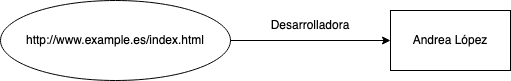
\includegraphics[scale=0.7]{../img/Diagrama-Nodo-Arco.png}
		\caption{Diagrama de nodo y arco simple que representa el ejemplo de setencia RDF.}
		\label{fig:Diagrama-Nodo-Arco}
	\end{figure}

	\fbox{\parbox{\textwidth}{
    \textbf{Nota:} La dirección de la flecja del arco simple es muy importante. El arco siempre debe de empezar en el sujeto y apunta hacia el objeto de la sentencia RDF. De manera general se puede usar la siguiente sentencia:

		\textbf{<Sujeto> TIENE <Predicado> <Objeto>}
}}

A partir del ejemplo comprendido de manera previa, se pueden especificar algunas características más para dicho ejemplo como:

\begin{verbatim}
	El indiviudo cuyo nombre es Andrea López, correo electrónico <andre@example.es>, 
	es la desarrolladores de la página web <http://www.example.es/index.html>.
\end{verbatim}

Teniendo esto en cuenta, la intención del ejemplo se basa en darle valor a la propiedad \textbf{desarrolladora} mediante una entidad estructurada. Por tanto, se puede observar a continuación el diagrama de nodo y arco simple que representa el ejemplo adjunto anteriormente:

\begin{figure}[H]
	\centering
	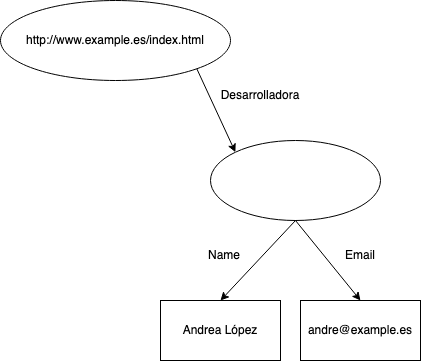
\includegraphics[scale=0.7]{../img/Propiedad-Estructurada.png}
	\caption{Diagrama de nodo y arco simple que representa el ejemplo de setencia RDF.}
	\label{fig:Diagrama-Nodo-Arco-2}
\end{figure}

\fbox{\parbox{\textwidth}{
	\textbf{Nota:} Se puede leer el diagrama anterior como http://www.example.es/index.html tiene la desarrolladora cualquiera y este cualquiera tiene el nombre Andrea López y el correo electrónico andre@example.es .
}}

Para finalizar, se puede implementar como ejemplo el uso de múltiples frases o sentecias RDF, por tanto, se tiene el siguiente ejemplo para ello:

\begin{verbatim}
	El individuo al que se refiere el identificador de empleado id 15151 se llama Andrea López y 
	tiene la dirección de correo electrónico <andre@example.es>. Este individuo creó el 
	recurso <http://www.example.es/index.html> y es la desarrolladora de este recurso.
\end{verbatim}

Con esto en mente, se implementad el siguiente \textbf{modelo RDF}:

\begin{figure}[H]
	\centering
	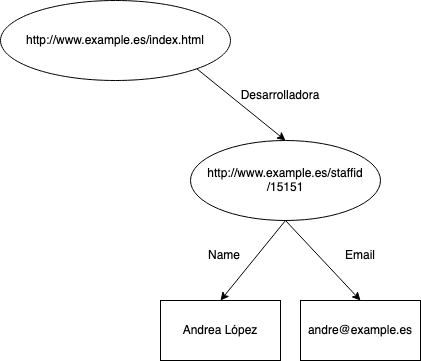
\includegraphics[scale=0.7]{../img/Modelo-RDF.png}
	\caption{Modelo RDF que representa el ejemplo de múltiples sentencias RDF.}
	\label{fig:Modelo-RDF}
\end{figure}

	\chapter{RDF y XML}
	SAMUEL
	\url{https://arxiu-web.upf.edu/hipertextnet/numero-1/rdf.html#2.2}

	\chapter{Principios de Linked Data según Tim Berners-Lee}
	SAMUEL

	\chapter{Proyecto Linking Open Data}
	Example....

	\chapter{Linked Open Data (LOD)}
	Example....

	\chapter{Relación entre Linked Data y Open Data}
	Example....

	\chapter{Linked Data y Web Semántica}
	Example....

	\chapter{Linked Data y Web 3.0}
	Example....

	\chapter{Beneficios de Linked Data}
	Example....

	\chapter{Problemas de Linked Data}
	Example....

	\chapter{Linked Data en bibliotecas}
	Example....

	\chapter{Linked Data en la actualidad}
	Example....

	\chapter{Conclusiones}
	Example....

	\begin{thebibliography}{99}
	\bibitem{1} CloudFlare. 2023.  ¿Qué es el modelo OSI?.  CloudFlare.  \url{https://www.cloudflare.com/es-es/learning/ddos/glossary/open-systems-interconnection-model-osi/}
	\bibitem{2} 12Características. 2023. HTTP (Características, concepto y funciones). 12Características. \url{https://www.12caracteristicas.com/http/}
	\bibitem{3} REDTECA. 2023. Protocolo HTTP. REDTECA. \url{https://redteca.com/hostings/http}
	\bibitem{4}OpenData Euskadi. 2023. RDF (Resource Description Framework). OpenData. \url{https://opendata.euskadi.eus/contenidos/informacion/opendata_rdf_euskadi/es_info/adjuntos/RDF.pdf}
	\bibitem{5} ARITMETICS. 2023. Qué es W3C. ARITMETICS. \url{https://www.arimetrics.com/glosario-digital/w3c}
	\bibitem{6} AWS. 2023. ¿Qué es XML?. Amazon. \url{https://aws.amazon.com/es/what-is/xml/}
	\bibitem{7}.  Eva Méndez. 2001. Resource Description Framework(RDF)	Especificación del Modelo y la Sintaxis. SIDAR. \url{http://www.sidar.org/recur/desdi/traduc/es/rdf/rdfesp.htm#basic}
	\bibitem{8} María Jesús Lamarca Lapuente. 2018. Hipertexto, el nuevo concepto de documento en la cultura de la imagen. Hipertexto. \url{http://www.hipertexto.info/documentos/rdf.htm}
	\end{thebibliography}

	\end{document}